\hypertarget{stm32f4xx__hal__cortex_8c}{}\section{Dokumentacja pliku S\+T\+M/\+W\+D\+S\+\_\+\+Kosc\+\_\+\+Linux/\+Drivers/\+S\+T\+M32\+F4xx\+\_\+\+H\+A\+L\+\_\+\+Driver/\+Src/stm32f4xx\+\_\+hal\+\_\+cortex.c}
\label{stm32f4xx__hal__cortex_8c}\index{S\+T\+M/\+W\+D\+S\+\_\+\+Kosc\+\_\+\+Linux/\+Drivers/\+S\+T\+M32\+F4xx\+\_\+\+H\+A\+L\+\_\+\+Driver/\+Src/stm32f4xx\+\_\+hal\+\_\+cortex.\+c@{S\+T\+M/\+W\+D\+S\+\_\+\+Kosc\+\_\+\+Linux/\+Drivers/\+S\+T\+M32\+F4xx\+\_\+\+H\+A\+L\+\_\+\+Driver/\+Src/stm32f4xx\+\_\+hal\+\_\+cortex.\+c}}


C\+O\+R\+T\+EX H\+AL module driver. This file provides firmware functions to manage the following functionalities of the C\+O\+R\+T\+EX\+:  


{\ttfamily \#include \char`\"{}stm32f4xx\+\_\+hal.\+h\char`\"{}}\newline
Wykres zależności załączania dla stm32f4xx\+\_\+hal\+\_\+cortex.\+c\+:\nopagebreak
\begin{figure}[H]
\begin{center}
\leavevmode
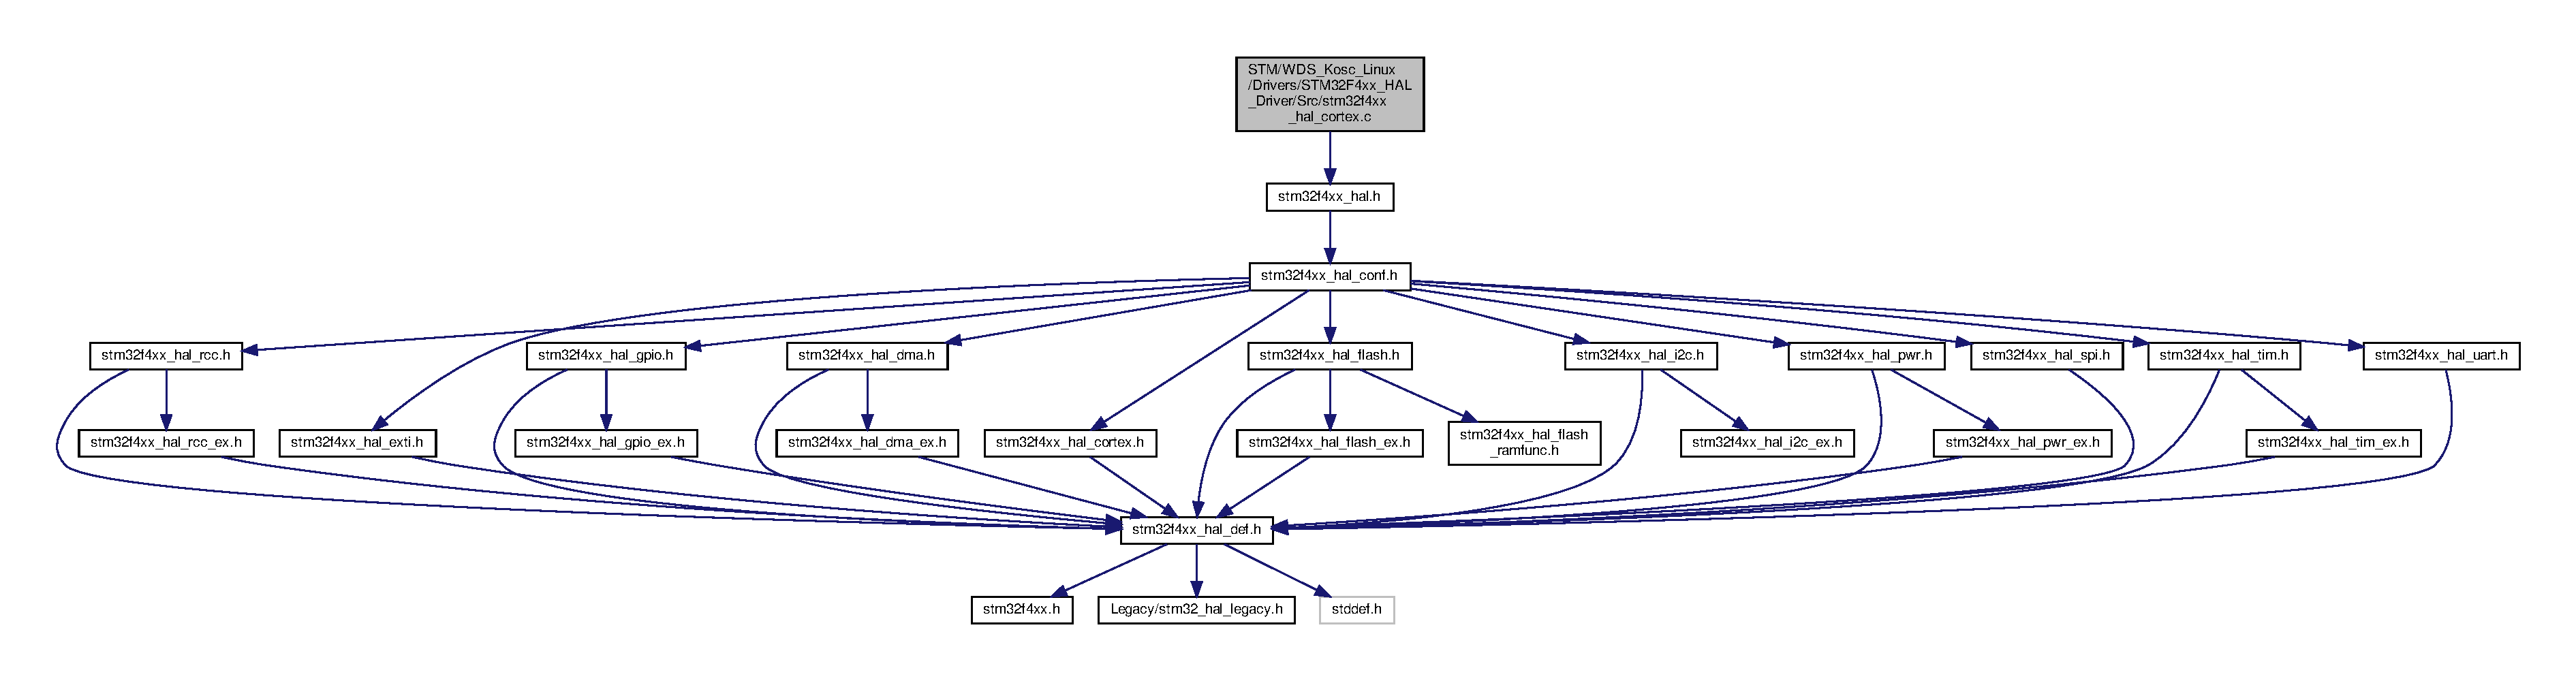
\includegraphics[width=350pt]{stm32f4xx__hal__cortex_8c__incl}
\end{center}
\end{figure}


\subsection{Opis szczegółowy}
C\+O\+R\+T\+EX H\+AL module driver. This file provides firmware functions to manage the following functionalities of the C\+O\+R\+T\+EX\+: 

\begin{DoxyAuthor}{Autor}
M\+CD Application Team
\begin{DoxyItemize}
\item Initialization and de-\/initialization functions
\item Peripheral Control functions
\end{DoxyItemize}
\end{DoxyAuthor}
\begin{DoxyVerb}==============================================================================
                      ##### How to use this driver #####
==============================================================================

  [..]  
  *** How to configure Interrupts using CORTEX HAL driver ***
  ===========================================================
  [..]     
  This section provides functions allowing to configure the NVIC interrupts (IRQ).
  The Cortex-M4 exceptions are managed by CMSIS functions.
 
  (#) Configure the NVIC Priority Grouping using HAL_NVIC_SetPriorityGrouping()
      function according to the following table.
  (#) Configure the priority of the selected IRQ Channels using HAL_NVIC_SetPriority(). 
  (#) Enable the selected IRQ Channels using HAL_NVIC_EnableIRQ().
  (#) please refer to programming manual for details in how to configure priority. 
    
   -@- When the NVIC_PRIORITYGROUP_0 is selected, IRQ preemption is no more possible. 
       The pending IRQ priority will be managed only by the sub priority.
 
   -@- IRQ priority order (sorted by highest to lowest priority):
      (+@) Lowest preemption priority
      (+@) Lowest sub priority
      (+@) Lowest hardware priority (IRQ number)

  [..]  
  *** How to configure Systick using CORTEX HAL driver ***
  ========================================================
  [..]
  Setup SysTick Timer for time base.
         
 (+) The HAL_SYSTICK_Config() function calls the SysTick_Config() function which
     is a CMSIS function that:
      (++) Configures the SysTick Reload register with value passed as function parameter.
      (++) Configures the SysTick IRQ priority to the lowest value 0x0F.
      (++) Resets the SysTick Counter register.
      (++) Configures the SysTick Counter clock source to be Core Clock Source (HCLK).
      (++) Enables the SysTick Interrupt.
      (++) Starts the SysTick Counter.
  
 (+) You can change the SysTick Clock source to be HCLK_Div8 by calling the macro
     __HAL_CORTEX_SYSTICKCLK_CONFIG(SYSTICK_CLKSOURCE_HCLK_DIV8) just after the
     HAL_SYSTICK_Config() function call. The __HAL_CORTEX_SYSTICKCLK_CONFIG() macro is defined
     inside the stm32f4xx_hal_cortex.h file.

 (+) You can change the SysTick IRQ priority by calling the
     HAL_NVIC_SetPriority(SysTick_IRQn,...) function just after the HAL_SYSTICK_Config() function 
     call. The HAL_NVIC_SetPriority() call the NVIC_SetPriority() function which is a CMSIS function.

 (+) To adjust the SysTick time base, use the following formula:
                          
     Reload Value = SysTick Counter Clock (Hz) x  Desired Time base (s)
     (++) Reload Value is the parameter to be passed for HAL_SYSTICK_Config() function
     (++) Reload Value should not exceed 0xFFFFFF\end{DoxyVerb}


\begin{DoxyAttention}{Uwaga}

\end{DoxyAttention}
\subsubsection*{\begin{center}\copyright{} Copyright (c) 2017 S\+T\+Microelectronics. All rights reserved.\end{center} }

This software component is licensed by ST under B\+SD 3-\/\+Clause license, the \char`\"{}\+License\char`\"{}; You may not use this file except in compliance with the License. You may obtain a copy of the License at\+: opensource.\+org/licenses/\+B\+S\+D-\/3-\/\+Clause 